\documentclass[border=10pt]{standalone}
\usepackage[european]{circuitikz}
\begin{document}
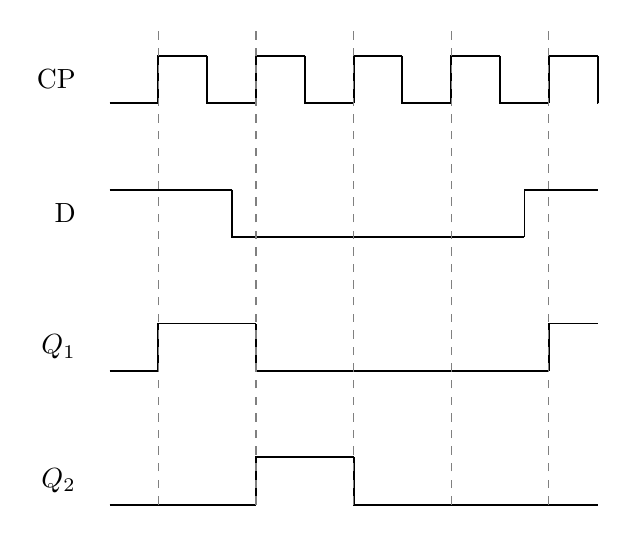
\begin{tikzpicture}[line width=0.7pt, font=\normalsize]

% 习题 8.9 答案波形：CP / Q₁ / Q₂ 三行
%   CP 五个脉冲（手绘无刻度，10 等分，沿位与页面内联 SVG 一致）：
%     ↑₁=1 ↓₁=2 ↑₂=3 ↓₂=4 ↑₃=5 ↓₃=6 ↑₄=7 ↓₄=8 ↑₅=9 ↓₅=10（单位：段）
%     实际页面 polyline：x 30/60/90/164/194/268/298/372/402/476/506/550
%     等分后沿位归一到 1,2,3,4,5,6,7,8,9,10 段（每脉冲 1 段高、1 段低）
%   D：0–↑₁ 高；D↓ 在 ↓₁–↑₂ 之间（取 2.5 段）；D↑ 在 ↓₄–↑₅ 之间（取 8.5 段）；末尾高
%   Q₁：↑₁ 置 1、↑₂ 置 0、↑₅ 置 1（页面结论）
%   Q₂：按 J=Q₁、K=Q̄₁ ⇒ Q₂*=Q₁，滞后一拍；高脉冲 ↑₂–↑₃（页面结论）
% 10 等分、无刻度、左端标 CP/D/Q、竖虚线五沿。

\def\seg{0.62}
\def\hi{0.6}
\def\total{6.2}

\newcommand{\wave}[3]{%
  \begin{scope}[yshift=#1cm]
    \node[anchor=east] at (-0.3,\hi/2) {#2};
    #3
  \end{scope}}

% CP：0 低 |1-2 高 |2-3 低 |3-4 高 |4-5 低 |5-6 高 |6-7 低 |7-8 高 |8-9 低 |9-10 高 |10 低收尾? 
% 页面 polyline 收尾 x=550,y55（低）→ 第5脉冲高在 9-10? 重新按页面：
% 段: 0-1 低, 1-2 高, 2-3 低, 3-4 高, 4-5 低, 5-6 高, 6-7 低, 7-8 高, 8-9 低, 9-10 高, 10-末 低
\wave{0}{CP}{%
  \draw (0,0) -- (\seg,0);
  \draw (\seg,0) -- (\seg,\hi) -- (2*\seg,\hi);
  \draw (2*\seg,\hi) -- (2*\seg,0) -- (3*\seg,0);
  \draw (3*\seg,0) -- (3*\seg,\hi) -- (4*\seg,\hi);
  \draw (4*\seg,\hi) -- (4*\seg,0) -- (5*\seg,0);
  \draw (5*\seg,0) -- (5*\seg,\hi) -- (6*\seg,\hi);
  \draw (6*\seg,\hi) -- (6*\seg,0) -- (7*\seg,0);
  \draw (7*\seg,0) -- (7*\seg,\hi) -- (8*\seg,\hi);
  \draw (8*\seg,\hi) -- (8*\seg,0) -- (9*\seg,0);
  \draw (9*\seg,0) -- (9*\seg,\hi) -- (10*\seg,\hi);
  \draw (10*\seg,\hi) -- (10*\seg,0) -- (\total,0);}

% D：0–2.5 高 |2.5–8.5 低 |8.5–末 高
\wave{-1.7}{D}{%
  \draw (0,\hi) -- (2.5*\seg,\hi);
  \draw (2.5*\seg,\hi) -- (2.5*\seg,0) -- (8.5*\seg,0);
  \draw (8.5*\seg,0) -- (8.5*\seg,\hi) -- (\total,\hi);}

% Q₁：↑₁(x=1) 置 1；↑₂(x=3) 置 0；↑₅(x=9) 置 1
\wave{-3.4}{$Q_1$}{%
  \draw (0,0) -- (\seg,0);
  \draw (\seg,0) -- (\seg,\hi) -- (3*\seg,\hi);
  \draw (3*\seg,\hi) -- (3*\seg,0) -- (9*\seg,0);
  \draw (9*\seg,0) -- (9*\seg,\hi) -- (\total,\hi);}

% Q₂：↑₂(x=3) 置 1；↑₃(x=5) 置 0（高脉冲 ↑₂–↑₃，滞后一拍）
\wave{-5.1}{$Q_2$}{%
  \draw (0,0) -- (3*\seg,0);
  \draw (3*\seg,0) -- (3*\seg,\hi) -- (5*\seg,\hi);
  \draw (5*\seg,\hi) -- (5*\seg,0) -- (\total,0);}

% 五条上升沿竖虚线（贯穿四行，画在波形之后）
\foreach \g in {1,3,5,7,9} {
  \draw[dashed, gray, line width=0.4pt] (\g*\seg,-5.1) -- (\g*\seg,0.95);
}

\end{tikzpicture}
\end{document}
